\def\anonymized{0} % uncomment to compile the non-anonymized version of the document
% \def\anonymized{1} % uncomment to compile the anonymized version of the document

\documentclass[11pt]{article}
\usepackage[utf8]{inputenc}
\usepackage[english]{babel}
\usepackage[a4paper, margin=1in]{geometry}
\usepackage[normalem]{ulem}
\usepackage{
    amsmath,amsthm,amscd,amsfonts,amssymb, 
    threeparttable,booktabs,pdflscape,tabularray,
    graphicx,float,hyperref,
    lineno,fancyhdr,
    natbib,
    setspace,siunitx,
    xr,appendix,
    codehigh
}
\UseTblrLibrary{booktabs}
\UseTblrLibrary{siunitx}
\newcommand{\tinytableTabularrayUnderline}[1]{\underline{#1}}
\newcommand{\tinytableTabularrayStrikeout}[1]{\sout{#1}}
\NewTableCommand{\tinytableDefineColor}[3]{\definecolor{#1}{#2}{#3}}


\newtheorem{theorem}{Theorem}
\newtheorem{proposition}{Proposition}
\newtheorem{lemma}{Lemma}
\newtheorem{corollary}{Corollary}
\newtheorem{conjecture}{Conjecture}
\theoremstyle{definition}
\newtheorem{definition}{Definition}
\newtheorem{assumption}{Assumption}
\newtheorem{axiom}{Axiom}
\newtheorem{hypothesis}{Hypothesis}
\theoremstyle{remark}
\newtheorem{remark}{Remark}

% \externaldocument{../appendix/main} % uncomment to tie to an external appendix (see appendix template; use relative paths)

\title{
    Title
    % \thanks{Acknowledgements}
}
\author{
    Romain Ferrali
    \thanks{
        Aix-Marseille University, CNRS, AMSE, France, {\tt \href{mailto:romain.ferrali@univ-amu.fr}{romain.ferrali@univ-amu.fr}.}
    }
}
\date{\today}

% ---- Publication ready manuscript has a fancy page header ----
\if\anonymized0
\pagestyle{fancy}
\fancyhf{}
\lhead{Title}
\rhead{
    Ferrali
}
\cfoot{\thepage}
\setlength{\headheight}{14pt}
\fi

% ---- Anonymized manuscript specific layout --- 
\if \anonymized1
\onehalfspacing % wider line spacing
\linenumbers % add line numbers
\fi

\begin{document}
\sloppy % avoid overfull hboxes

\if\anonymized0
    \maketitle
    %TC:ignore
    \begin{abstract}
        A terrific paper likely to get you the Nobel prize.
    \end{abstract}
    %TC:endignore
\fi

\section{Introduction}

This is a nice paper in the style of \citet{Ferrali}.

\begin{table}[H]
    \centering
    \input{./assets/tables/table.tex}
    \caption{A table generated with R}
    \label{tab:r_table}
\end{table}

\begin{figure}
    \centering
    \includegraphics{./assets/figures/figure.pdf}
    \caption{A figure generated with R}
    \label{fig:r_figure}
\end{figure}

\begin{figure}
    \centering
    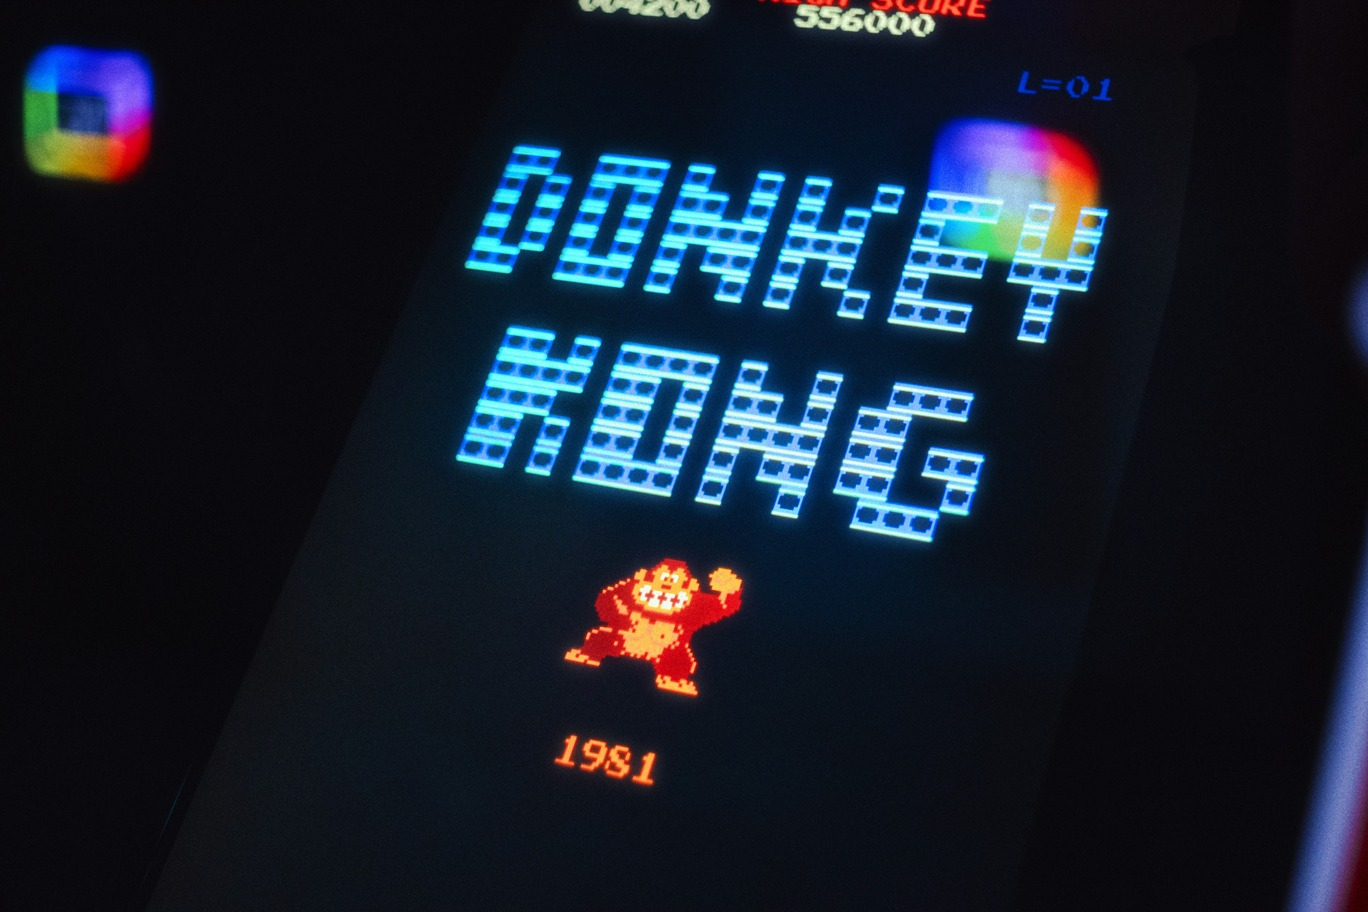
\includegraphics[width=\textwidth]{./assets/static/dk.jpg}
    \caption{A static figure. Photo by \href{https://unsplash.com/@ninjason?utm_content=creditCopyText&utm_medium=referral&utm_source=unsplash}{Jason Leung} on \href{https://unsplash.com/photos/donkey-kong-arcade-game-screen-with-1981-date-c5tiCWrZADc?utm_content=creditCopyText&utm_medium=referral&utm_source=unsplash}{Unsplash}
    }
    \label{fig:nice_figure}
\end{figure}

% ---- Bibliography ----
\newpage
%TC:ignore
\bibliographystyle{aer}
\bibliography{library}
%TC:endignore

\newpage

% ---- Appendix ----
%TC:ignore
% \appendix
% \appendixpage
% \addappheadtotoc
% Appendix content
%TC:endignore

\end{document}